\documentclass[11pt]{article}
\usepackage{amssymb,amsmath}
\usepackage{color,soul}
\usepackage{tikz,ifthen,calc}
\usetikzlibrary{positioning}
\usetikzlibrary{shapes}
\usetikzlibrary{shapes.symbols,patterns}
\usetikzlibrary{calc,through,backgrounds}
\usetikzlibrary{decorations.pathreplacing}
\usetikzlibrary{shapes.geometric, arrows}

\begin{document}

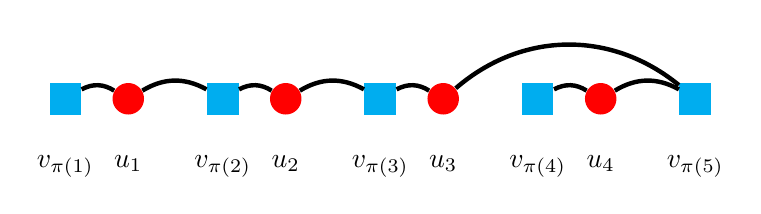
\begin{tikzpicture}[scale=0.4]	
\def\pathlen{5}
\def\pathspacing{5}
\pgfmathtruncatemacro{\plenplusone}{\pathlen + 1}
			
\foreach \x in {1,...,\pathlen} {
				
	\pgfmathtruncatemacro{\xcoord}{\x * \pathspacing}
	\node [label={[below = 8mm]$v_{\pi(\x)}$},minimum size= 4mm,fill=cyan] (v\x) at (\xcoord,0)  {};
			}
\foreach \x in {1,...,4} {
				
	\pgfmathtruncatemacro{\xcoord}{2 + \x *  \pathspacing}
	\node [label={[below = 8mm]$u_{\x}$},minimum size= 4mm,fill=red,circle] (u\x) at (\xcoord,0)  {};
			}
		
	\path [draw=black,ultra thick] (v1) [bend left=30] edge (u1);	
	\path [draw=black,ultra thick] (u1) [bend left=30] edge (v2);
	\path [draw=black,ultra thick] (v2) [bend left=30] edge (u2);		
	\path [draw=black,ultra thick] (u2) [bend left=30] edge (v3);
	\path [draw=black,ultra thick] (v3) [bend left=30] edge (u3);
	\path [draw=black,ultra thick] (u3) [bend left=40] edge (v5);
	
	\path [draw=black,ultra thick] (v4) [bend left=30] edge (u4);
	\path [draw=black,ultra thick] (u4) [bend left=30] edge (v5);

\end{tikzpicture}

\end{document}